\section{RC-Glied}

\subsection{Arbeitsgrundlagen}

\subsection{Durchf\"{u}hrung}

\subsubsection*{Versuchsanordnung}

\subsubsection*{Messergebnisse}

\bgroup
    \setlength\tabcolsep{8mm}
    \begin{center}
        \begin{threeparttable}
            \caption{Gemessene Gr\"ossen}
            \begin{tabular}{ccc}
                \toprule
                $f(Hz)$  &  $U_a(V)$    &  $\phi$ \\
                \midrule
                100      & 4.000        & -3.24   \\
                500      & 3.800        & -16.9   \\
                1000     & 3.300        & -31.3   \\
                1500     & 2.800        & -43.6   \\
                5000     & 1.140        & -72.4   \\
                10000    & 0.580        & -82.5   \\
                100000   & 0.075        & -90.0   \\
                1592     & 2.700        & -44.0   \\
                \bottomrule
            \end{tabular}
            \begin{tablenotes}
                \small
                \item Messprotokoll ``Tiefpass''
                \item Datum: 1. Okt. 1999
                \item Versuchsleiterin: Ruth Metzler
                \item \textbf{Hinweis:} Daten wurden vom Auftragsdokument kopiert.
            \end{tablenotes}
        \end{threeparttable}
    \end{center}
\egroup


\subsubsection*{QtiPlot}

\begin{figure}[H]
    \center
    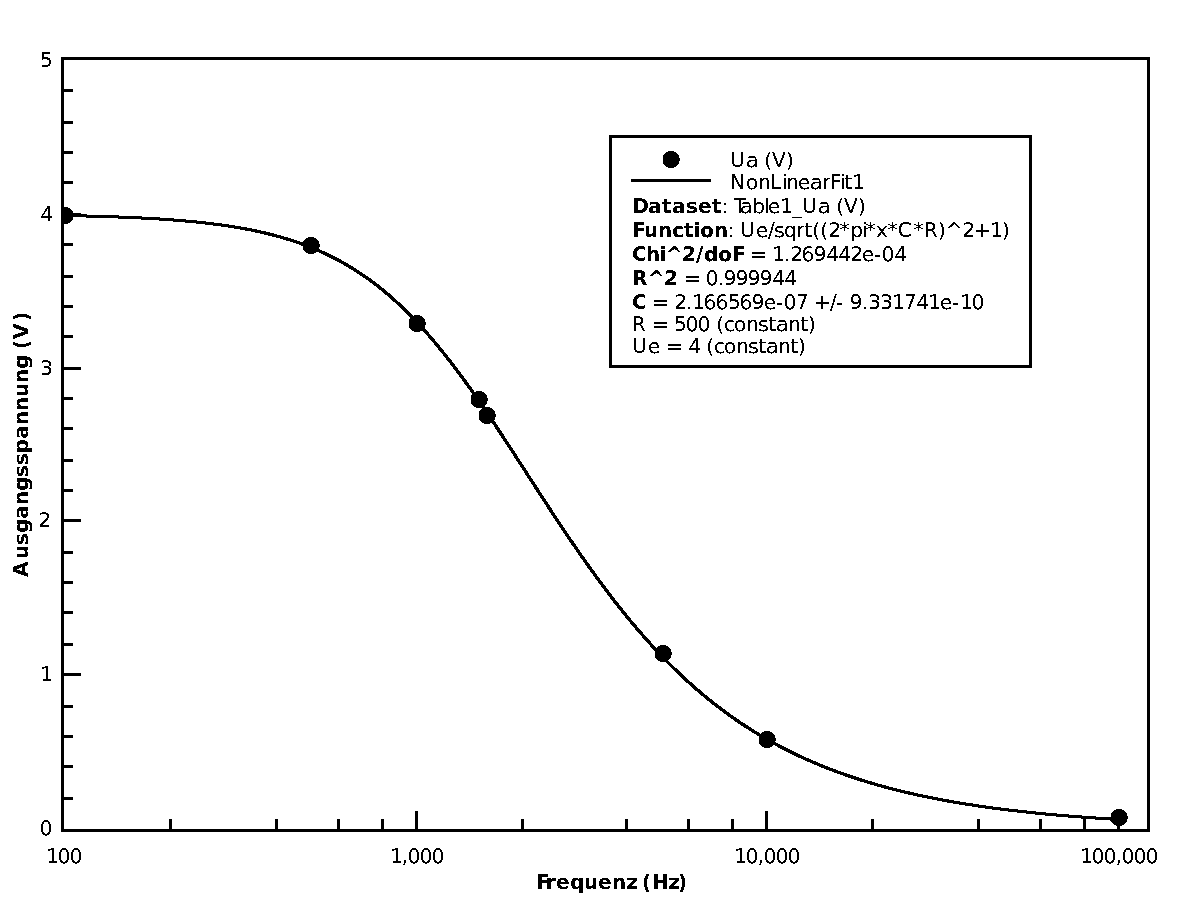
\includegraphics[width=.8\textwidth]{qtiplot/rc-ua}
    \caption{Nicht-lineare Regression zur Bestimmung von $C$ anhand der Ausgangsspannung}
    \label{fig:rc-ua}
\end{figure}

\begin{figure}[H]
    \center
    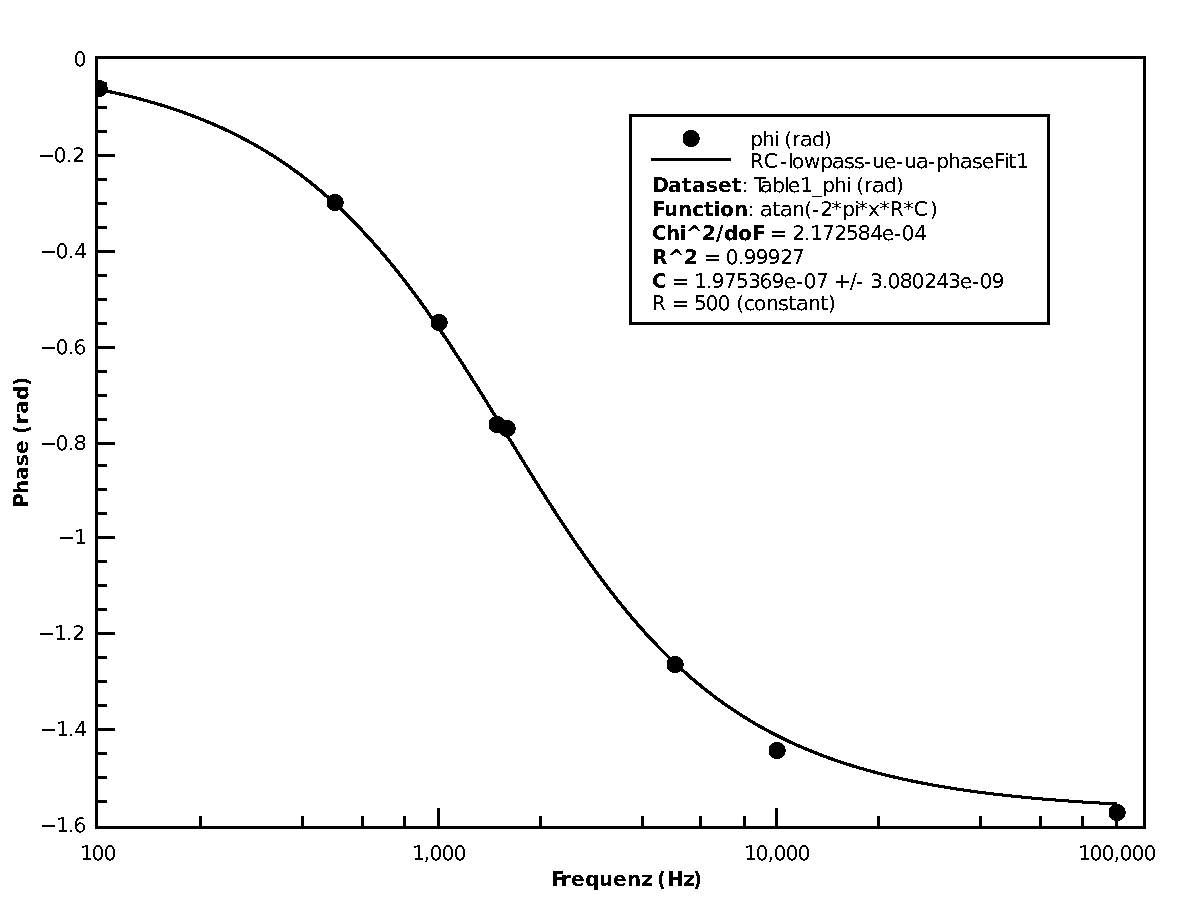
\includegraphics[width=.8\textwidth]{qtiplot/rc-phase}
    \caption{Nicht-lineare Regression zur Bestimmung von $C$ anhand der Phase}
    \label{fig:rc-phase}
\end{figure}

